\chapter{Antecedentes}
En este capítulo se describirán los aspectos generales de los principales componentes del estudio. Primero se describirán diferentes algoritmos básicos usados para clasificación de series temporales. Tras esto se explicarán qué son las LSTM, su funcionamiento y estructura. Por último, se describirá el problema de desbalanceo de clases y diferentes enfoques para solucionarlo.\newline

\section{Clasificación de series temporales. Algoritmos Básicos}
En esta sección se describirán algoritmos básicos para predicción de series temporales, así como algoritmos utilizados cuando se trabaja con series temporales de clasificación.\newline

\subsection{Series temporales de regresión.}
Cuando tratamos con series temporales nos encontramos con un problema de regresión clásico; en principio, se puede intentar utilizar métodos clásicos de regresión, pero normalmente no suelen dar buenos resultados. Para este tipo de problemas, el modelo más utilizado es ARIMA.\newline

ARIMA se trata de un modelo clásico para series temporales. Dicho modelo se trata de una combinación de otros modelos, modelos autoregresivos (AR, AutoRegressive) y modelos de medias móviles (MA, Moving Averages).Además de esto, incorporan la diferenciación de series temporales dentro del propio modelo.\newline

En un modelo AR; a diferencia de un modelo de regresión normal, donde se utiliza una combinación lineal de características para predecir una variable; se utiliza una combinación lineal de los valores anteriores de dicha variable. Un modelo AR de order $p$, al que nos referimos como $AR(p)$ se define de la siguiente forma:\newline
$$ y_t = c + \phi_1 y_{t-1} + \phi_2 y_{t-2} + ... + \phi_p y_{t-p} + \varepsilon_t $$

Donde $\varepsilon_t$ es ruido blanco, el ruido blanco es un tipo de serie temporal donde su varianza es siempre la misma y cada valor no tiene correlación con el resto de valores de la serie. Los valores $y_{t-1}, ..., y_{t-p}$ son los $p$ valores anteriores en la serie que se utilizan para calcular el valor actual. Los valores $\phi_1, ..., \phi_p$ son parámetros que el modelo modifica para ajustarse a la serie; $c$ es un término independiente.\newline

\begin{figure}[h]
	\centering
	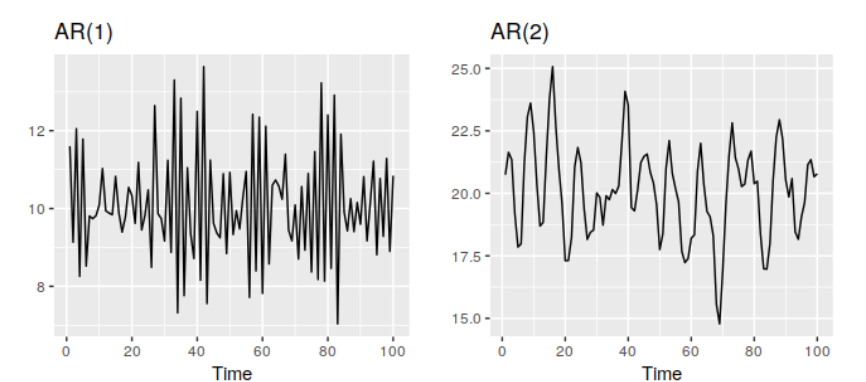
\includegraphics[width=100mm]{imagenes/autoregression_example.png}
	\label{fig:211}
	\caption{Diferentes modelos AR.}
\end{figure}
\verticalspace

Un modelo MA, a diferencia de un modelo AR utiliza los errores de predicciones anteriores para generar un modelo de regresión. Un modelo MA con grado $q$, al que llamaremos $MA(q)$ se define de la siguiente manera:
$$ y_t = c + \varepsilon_t + \theta_1 \varepsilon_{t-1} + \theta_2 \varepsilon_{t-2} + ... + \theta_q \varepsilon_{t-q}$$

Donde $\varepsilon_t$ es ruido blanco. Al igual que en el modelo anterior, $\theta_1, ..., \theta_q$ son parámetros que el modelo entrena para ajustarse a una serie temporal.

\begin{figure}[h]
	\centering
	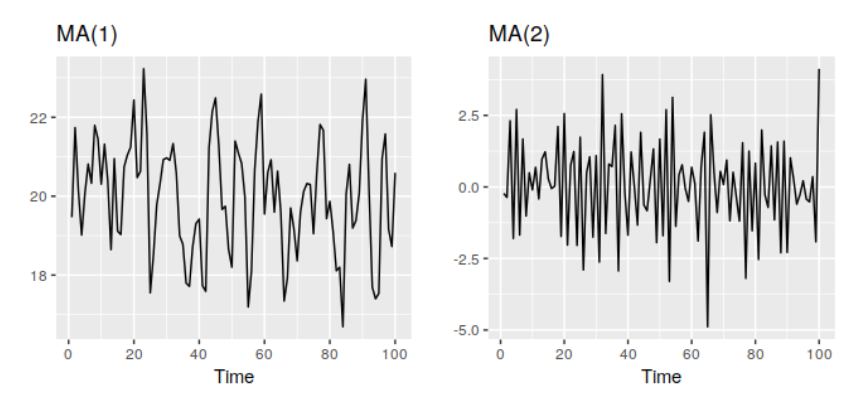
\includegraphics[width=100mm]{imagenes/moving_averages_example.png}
	\label{fig:212}
	\caption{Diferentes modelos MA.}
\end{figure}
\verticalspace

El último concepto que añade ARIMA es la diferenciación. La diferenciación es un proceso que se aplica a series temporales que no son estacionarias. Una serie temporal estacionaria es aquella cuya media y varianza se mantienen constantes. La diferenciación se trata del calculo de la diferencia entre observaciones consecutivas de la serie; por ejemplo una diferenciación de grado 1 en una serie se puede definir como $ y'_t = y_t - y_{t-1}$ y de grado 2 como $y''_t = y'_t - y'_{t-1} = y_t - 2y_{t-1} + y_{t-2}$.\newline

Combinando la diferenciación junto con los modelos AR y MA en un único modelo, se obtiene un modelo ARIMA. Un modelo ARIMA puede expresarse de la siguiente manera.
$$ y'_t = c + \phi_1 y'_{t-1} + ... + \phi_p y'_{t-p} + \theta_1 \varepsilon_{t-1} + ... + \theta_q \varepsilon_{t-q} + \varepsilon_t $$

Donde $y'_t$ es la serie diferenciada. De forma general, un modelo ARIMA se representa como $ARIMA(p,d,q)$ donde $p$ representa el grado del modelo AR, $d$ representa el grado de la diferenciación a la serie y $q$ representa el grado de del modelo MA. Si $p$ o $q$ son 0, entonces nos encontramos con un modelo MA o AR, dependiendo cual es 0.\newline

\begin{figure}[h]
	\centering
	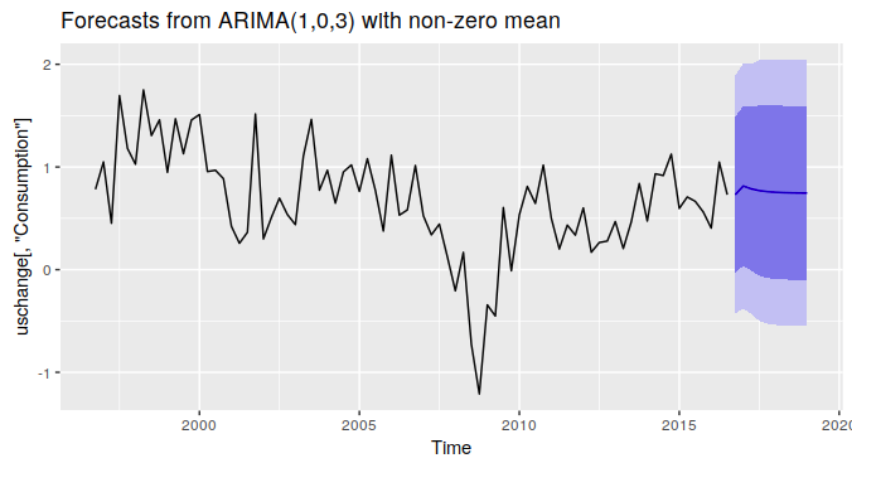
\includegraphics[width=100mm]{imagenes/arima_example.png}
	\label{fig:213}
	\caption{Ejemplo predicción con modelo ARIMA.}
\end{figure}
\newpage
\subsection{Series temporales de clasificación}
En el apartado anterior se ha descrito modelos utilizados cuando se estudian series temporales de regresión; en este aparatado se verán diferentes modelos utilizados cuando se estudian series temporales de clasificación.\newline

Las series temporales de clasificación tienen propiedades que hacen que ciertos aspectos del preprocesamiento haya que abarcarlos de forma diferente a diferencia de otro tipo de problemas; sin embargo, los métodos que se utilizan para su clasificación son los mismo que para cualquier otro tipo de problema de clasificación.\newline

Los métodos más utilizados, a parte de las redes neuronales que no se discutirán en este apartado; son SVM, RandomForest y Boosting. A continuación, se describirá el funcionamiento de estos algoritmos.\newline

\subsubsection{SVM}
El SVM (Support Vector Machine, Máquinas de Soporte Vectorial en español) fue introducido en 1992. Las SVM son un caso particular de \say{Kernel Machines} (KM). Este tipo de algoritmos utilizan el producto escalar de los datos de entrada, de esta forma, el producto escalar se usa como una forma de establecer una similitud entre los elementos.\newline

Con este producto escalar, se puede definir un hiperplano como $<x,w> + b = 0$; modificando el valor de $w$, se puede adaptar dicho hiperplano para separar mejor los datos, un ejemplo clásico de esto es el perceptron.\newline

\begin{figure}[h]
	\centering
	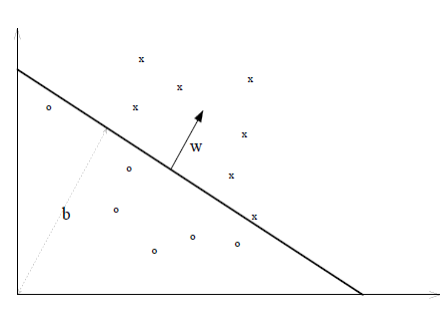
\includegraphics[width=80mm]{imagenes/perceptron_example.png}
	\label{fig:214}
	\caption{Ejemplo de hiperplano.}
\end{figure}
\newpage

Para obtener un buen valor de $w$, se puede utilizar una combinación lineal de los datos de entrada junto con un coeficiente que refleje su dificultad, $ w = \sum \alpha_i y_i x_i $. De esta forma, se puede representar ese hiperplano como $\sum \alpha_i y_i <x_i,x> + b$; para entrenar y ajustar este hiperplano simplemente se necesita modificar $\alpha_i$, si $f(x) = \sum \alpha_i y_i <x_i,x> + b <= 0$ entonces $\alpha_i = \alpha_i + \eta$. Gracias a esta nueva representación, la función de decisión (hiperplano) solo necesita los datos de entrada.\newline

La representación dual es la primera características de los SVM. El problema es que hasta ahora se han utilizado una separación lineal de los datos y en muchos casos los datos no son linealmente separables o existe ruido. La solución que da SVM para este problema es trasladar los datos, que no son linealmente separables a otro espacio donde sí lo sean, para ello utiliza los kernels.\newline

Un kernel es una función que devuelve el valor del producto escalar entre los datos llevados a otro espacio. Se puede representar de la siguiente forma.
$$ K(x_1,x_2) = <\phi(x_1), \phi(x_2)> $$

Donde $x_1, x_2$ son datos en el espacio original y $\phi$ representa la transformación para llevar un dato a otro espacio. Gracias a los kernels no es necesario saber la transformación $\phi$, además, a partir de este momento en la función del hiperplano se puede sustituir el producto escalar por la función kernel.\newline

Existen diferentes tipos de kernels, como por ejemplo el polinomial o el radial. A continuación se muestra un ejemplo de proyección en el espacio.\newline

\begin{figure}[h]
	\centering
	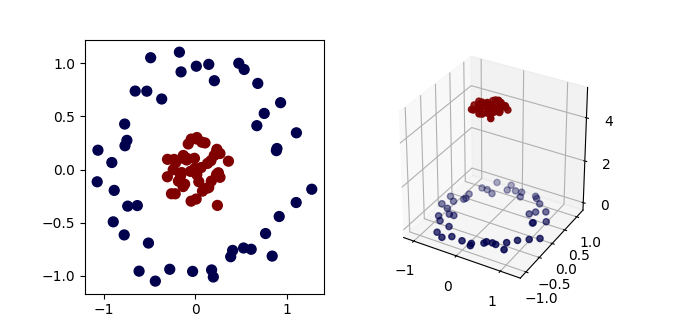
\includegraphics[width=100mm]{imagenes/svm_kernel_example.png}
	\label{fig:215}
	\caption{Ejemplo de proyección.}
\end{figure}
\newpage
Por último, la última características de las SVM es que tiene la capacidad
de maximizar el margen, es decir, de entre todos los hiperplanos que separan las dos clases, SVM se queda con aquel que maximiza la distancia a las dos clases, de esta forma se minimiza el riesgo de sobreaprendizaje.\newline

\subsubsection{RandomForest}
RandomForest es uno de los métodos clásicos que forma parte del estado del arte para algoritmos de clasificación. RandomForest se trata de un multiclasificador, es decir, es un modelo formado por varios modelos más simples; en el caso de RandomForest se utilizan árboles de clasificación.\newline

Los árboles de clasificación son un algorimto clásico de clasificación. El proceso que realiza un árbol de clasificación es dividir el espacio del problema hasta que llega decisión. El proceso que sigue para generar el árbol es el siguiente.\newline

Primero se busca el atributo que mejor separe las clases sobre el conjunto de datos entero (nodo raíz). Segundo, se divide el conjunto de datos según el atributo elegido y se elimina este. Este proceso se repite en cada nodo hasta que todos los elementos en ese elemento sea de la misma clase. El proceso se repite hasta que todas las ramas del árbol llegan a una solución.\newline

Para decidir que atributos son los que mejor separan las clase existe diferentes medidas como por ejemplo el índice GINI, Entropía, Ganancia de información o el Ratio de Gananacia. Las medidas GINI y Entropía miden interés en un atributo a partir de la frecuencia relativa entre clases para la partición de dicho atributo, la Ganancia mide la reducción en la Entropía al realizar una partición, el Ratio de Ganancia mide la Ganancia dividido entre el número de particiones que se realizan al particionar con ese atributo.\newline
\newpage
\begin{figure}[h]
	\centering
	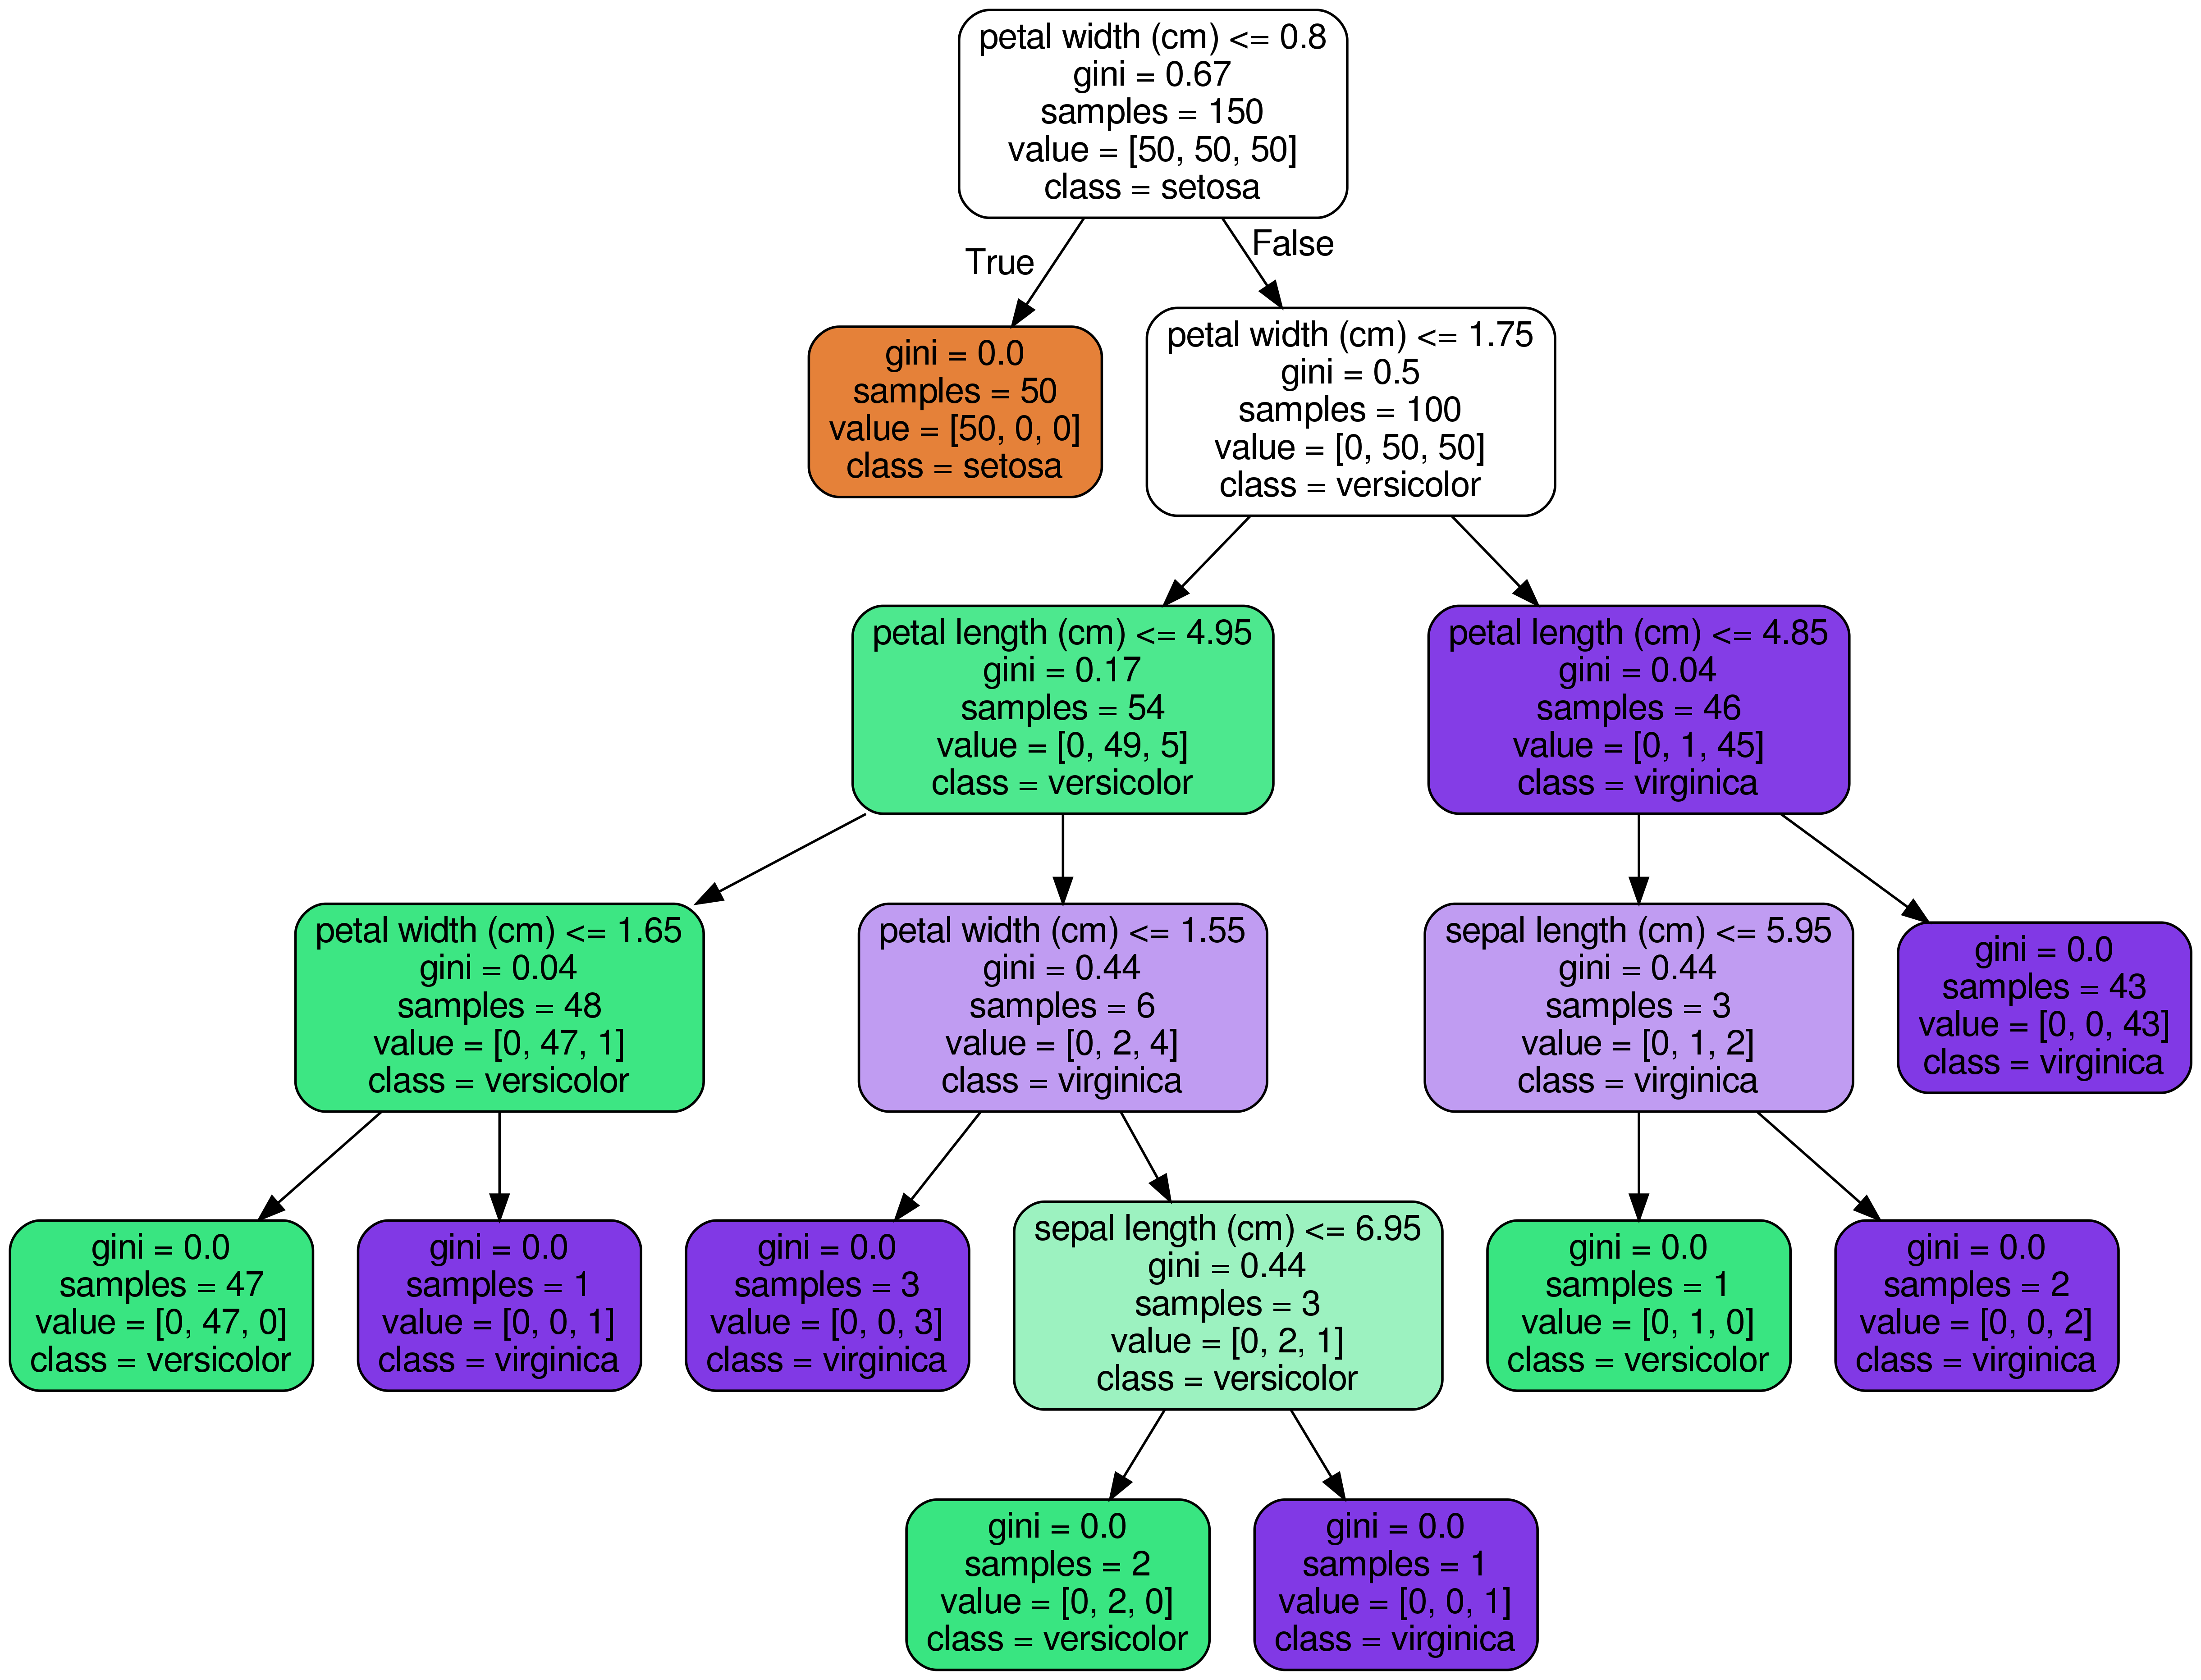
\includegraphics[width=100mm]{imagenes/tree_example.png}
	\label{fig:216}
	\caption{Ejemplo de árbol de clasificación.}
\end{figure}
\verticalspace

RandomForest crea un conjunto de árboles de clasificación para realizar su decisión; una vez creados los árboles, se decide la clase final mediante voto. Para generar los árboles se utiliza \textit{Bagging}. Para cada uno de los árboles, se eligen $m$ atributos y un subconjunto de instancias del conjunto de datos, de esta forma se obtiene modelos más simples que pueden aprender mejor ciertos atributos que si se creara un solo árbol de decisión.\newline

\subsubsection{Boosting}
Boosting, al igual que RandomForest se trata de un multiclasificador, aunque su enfoque es diferente. Boosting puede utilizarse tanto con árboles de decisión como con otros algoritmos.\newline

A diferencia de RandomForest, donde cada árbol que se genera es independiente, en Boosting cada árbol o clasificador que se genera utiliza información de los árboles que se han creado anteriormente.\newline

El algorimto más conocido de Boosting es AdaBoost. AdaBoost sigue el siguiente proceso para crear $N$ clasificadores. 
\begin{itemize}
	\item Primero, elige un subconjunto de instancias del conjunto de datos según su peso y entrena un clasificador simple.\newpage
	\item Segundo, prueba el clasificador sobre el conjunto de datos completo y aumenta el peso de aquellos datos mal clasificados y reduce el de aquellos bien clasificados.
	\item Por último, asocia al clasificador entrenado un peso/importancia basada en el error cometido.
\end{itemize}
\verticalspace

Una vez creados los $N$ clasificadores, la clase final se decide mediante una combinación lineal de la salida de cada clasificador y su importancia.\newline

\begin{figure}[h]
	\centering
	\begin{subfigure}{.4\textwidth}
		\centering
		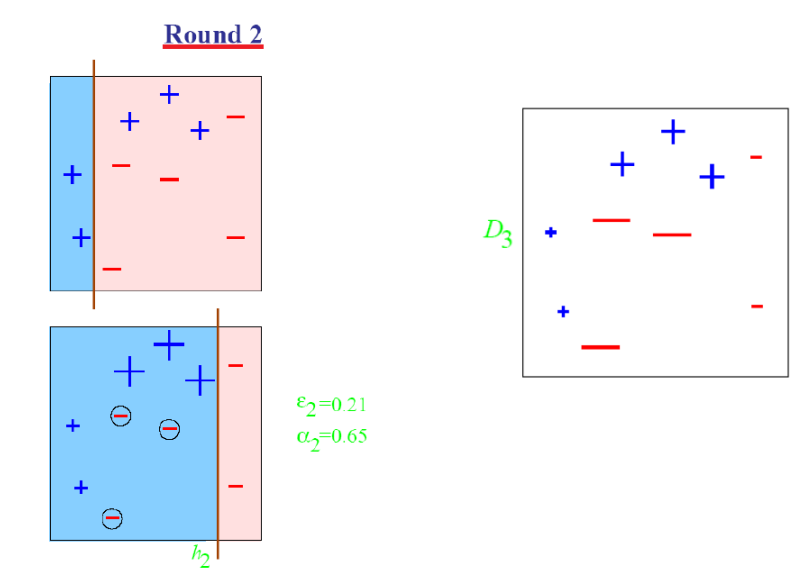
\includegraphics[width=50mm]{imagenes/boosting_2.png}
	\end{subfigure}
	\hspace{0.01in}
	\begin{subfigure}{.4\textwidth}
		\centering
		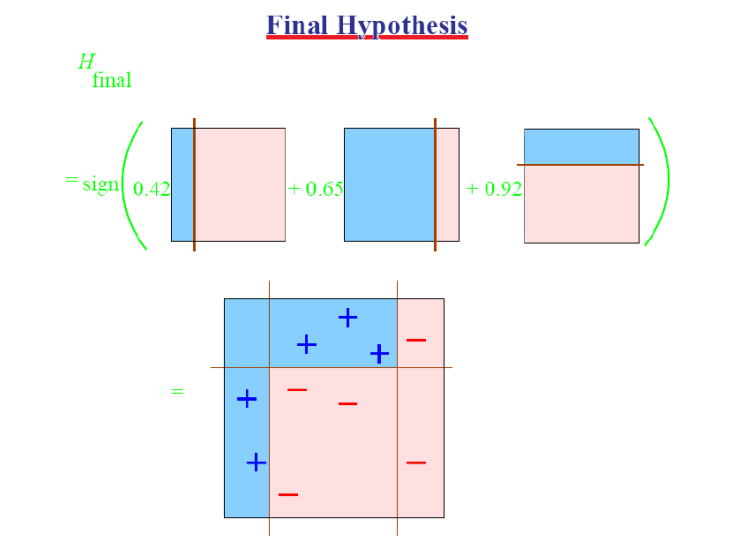
\includegraphics[width=50mm]{imagenes/boosting_final.png}
	\end{subfigure}
	\label{fig:217}
	\caption{Ejemplo funcionamiento AdaBoost.}
\end{figure}
\verticalspace

Para este estudio, el algoritmo que se utilizará es XGBoost; este es un algoritmo de Boosting, específicamente Gradient Boosted Trees. Este algoritmo utiliza el Boosting para generar nuevos árboles que puedan predecir la clase de los errores que han cometido árboles anteriores. Para minimizar la pérdida al añadir nuevos modelos se utiliza gradiente descendiente.\newline

XGBoost añade también el concepto de regularización a los Gradient Boosted Trees. La que es un mecanismo para evitar el sobreaprendizaje, para conseguir esto se mide la complejidad del modelo, de forma que se premian modelos más sencillos. XGBoost, a parte de optimizar la pérdida para conseguir mejores modelos, optimiza la regularización para obtener modelos más sencillos. Esto hace que pueda producir mejores resultados mejores que los Gradient Boosted Trees, ya que modelos más sencillos suelen generalizar mejor y por lo tanto sufrir menos sobreaprendizaje y siendo más estables.

\newpage
\section{LSTM}
Las LSTM ( Long Short-Term Memory ) son un tipo de red neuronal recurrente; este tipo de red es capaz de procesar de procesar secuencias de datos, como por ejemplo vídeos o frases. Este tipo de red neuronal se inventaron para ser usadas en problemas donde la información que se procesa es dependiente de información anteriormente procesada, y esta relación debe ser recordada hasta que deje de ser útil. Actualmente las redes con LSTM se utilizan en diversas tareas, como por ejemplo reconocimiento del habla, traducción, etc.\newline

Una unidad de LSTM o una neurona de LSTM tiene la siguiente estructura:
\begin{itemize}
	\item Puerta de entrada.
	\item Puerta de salida.
	\item Puerta de olvido.
	\item Célula.
\end{itemize}
\vspace{0.09in}
La célula es la encargada de almacenar información; el valor de la célula depende de los valores de las puertas de entrada, salida y olvido. Además, los valores de dichas puertas van cambiando en cada instante de tiempo. En la siguiente imagen se puede ver una representación de las estructura de una LSTM.\newline

\begin{figure}[h]
	\centering
	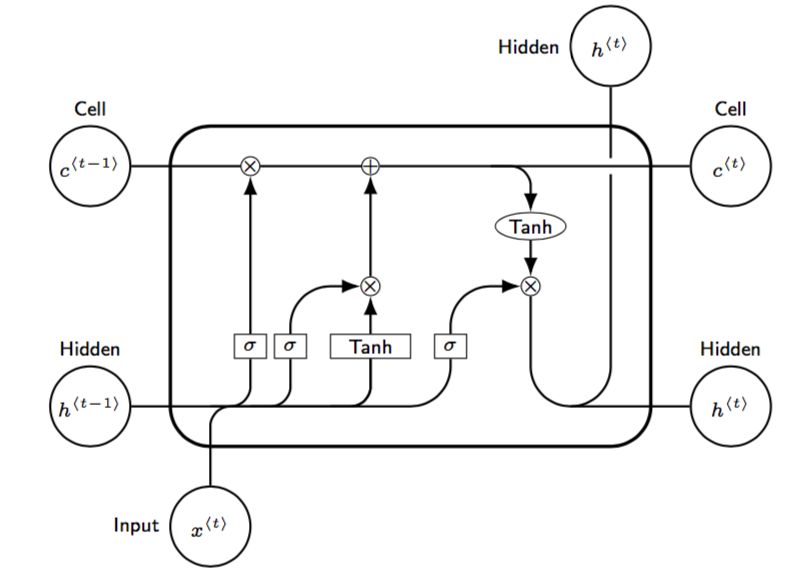
\includegraphics[width=120mm]{imagenes/lstm-struct.png}
	\label{fig:22}
	\caption{Estructura de una LSTM.}
\end{figure}
\vspace{0.09in}
La puerta de olvido tiene como función olvidar información anterior dependiendo de la información actual, dicha función podría expresarse de la siguiente forma.

$$ f^{(t)} = \sigma( W_f[h^{(t-1)}, x(t)] + b_f) $$

Donde:
\begin{itemize}
	\item $x^{(t)}$: entrada de la puerta en el momento $t$.
	\item $h^{(t-1)} $: valor de la salida de la célula en el instante anterior.
	\item $W_f $: matriz de pesos de la puerta de olvido.
	\item $b_f $: sesgo de la puerta de olvido.
	\item $\sigma$: función de activación (valores entre 0 y 1) de la puerta de olvido.
\end{itemize}
\vspace{0.09in}
La puerta de entrada tiene como función aprender los parámetros de entrada para su composición con el estado de la LSTM. PAra ello se debe calcular el estado de la LSTM y seleccionar la información que se utilizará para actualizar el estado. Esto se puede expresar mediante las siguientes funciones:\newline
$$ i^{(t)} = \sigma(W_i[h^{(t-1)}, x^{(t)}] + b_i) $$
$$ s'^{(t)} = \tanh(W_s[h^(t-1), x^{(t)}] + b_s) $$

Donde:
\begin{itemize}
	\item $s'^{(t)}$:estado local de la LSTM, sin tener en cuenta el estado anterior.
	\item $W_i$: matriz de pesos de la puerta de entrada.
	\item $W_s$: matriz de pesos del estado de la LSTM.
	\item $b_i $: sesgo de la puerta de entrada.
	\item $b_s$: sesgo del estado.
\end{itemize}
\verticalspace
Tras esto, se calcula el nuevo estado de la LSTM de la siguiente forma:\newline
$$ s^{(t)} = f^{(t)}s^{(t-1)} + i^{(t)} s'^{(t)} $$
De esta forma, el estado se forma con una parte del estado anterior, la que no se olvida; y con la composición de la entrada con el estado local ( $s'^{(t)}$ ).
\verticalspace

La puerta de salida es la encargada de aprender los parámetros de salida, esto puede expresarse mediante la siguiente función:\newline
$$ o^{(t)} = \sigma(W_o[h^{(t-1)}, x^{(t)}] + b_o) $$
Por último, la salida se calcula como:\newline
$$h^{(t)} = o^{(t)}\tanh(s^{(t)}) $$

La función para calcular la salida puede ser otra, como ReLu; las funciones de activación de las puertas también pueden ser otras.\newline

Como puede verse, las LSTM son capaces de guardar información relevante durante un largo periodo de tiempo y eliminar la información poco importante; por ello, son muy utilizadas en problemas con series temporales, ya que la información en un momento t es dependiente de la información que había en instantes anteriores y las LSTMs son capaces de detectar dicha dependencia y aprenderla.\newline

Las LSTM son un tipo de red recurrente, por lo que se pueden construir arquitecturas basadas en una LSTM que procesa la secuencia de izquierda a derecha y otra de derecha a izquierda; a estas estructuras se les llama LSTM bidireccionales, en la siguiente imagen se muestra un ejemplo de esta estructura.\newline
\newpage

\begin{figure}[h]
	\centering
	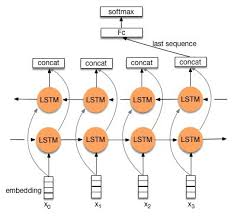
\includegraphics[width=85mm]{imagenes/bidi-lstm.jpg}
	\label{fig:23}
	\caption{Ejemplo de estructura de LSTM bidireccional.}
\end{figure}
\verticalspace
Gracias a este tipo de estructuras pueden resolverse problemas donde la importancia/sentido de un dato no depende de datos anteriores sino por información posterior; por ejemplo, el significado de una palabra puede ser diferente dependiendo de las palabras siguientes que haya en una secuencia y no en las anteriores.
\newpage
\section{Clasificación con clases no balanceadas}
El problema de desbalanceo de clases es un tipo de problema que aparece en problemas de clasificación. el desbalanceo de clases ocurre cuando el número de elementos de una clase es mucho mayor que el número de elementos de la otra clase; a esta clase se le llama clase minoritaria. En la siguiente imagen se puede ver un ejemplo en 2D de un problema de desbalanceo de clases.\newline

\begin{figure}[h]
	\centering
	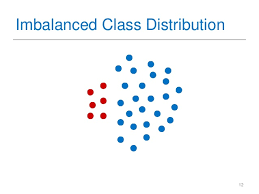
\includegraphics[width=85mm]{imagenes/imbalance_class.png}
	\label{fig:24}
	
\end{figure}
\verticalspace

El principal problema que tiene el desbalanceo de clases es que afecta a la capacidad de aprendizaje de la mayoría de los modelos de minería de datos actuales, exceptuando algunos como los árboles de decisión, aunque también trabajan mejor si no hay desbalanceo. Además, si el desbalanceo es muy grande es posible que los modelos no aprendan directamente la clase minoritaria.\newline

Otro problema es que afecta a las medidas utilizadas normalmente en problemas de clasificación como es el Accuracy; esta medida representa el número de elementos bien clasificados sobre el total de elementos; si por ejemplo la clase minoritaria representa el 0.1\% de los datos y un clasificador predijera todos los datos como elementos de la clase mayoritaria, su Accuracy sería del 99.9\%; por ello, se debe utilizar otras medidas. Las medidas usuales son Precision, Recall, AUC, G-Mean, F1-Score, etc; todas estas medidas tienen en cuenta la clase minoritaria de forma que si ocurre lo anterior su valor sea bajo.\newline

Como solución al problema del desbalanceo existen dos propuestas, una basada en modificación de algoritmos y otra basada en modificación del conjunto de datos.
\subsection{Técnicas basadas en modificación del algoritmo}
Este enfoque se centra en modificar clasificadores ya existentes para aliviar el sesgo hacia la clase mayoritaria en vez de alterar el conjunto de datos. Esto requiere un buen conocimiento interno del modelo que se quiere modificar y saber las razones por las cuales falla al identificar la clase minoritaria.\newline

Modificar un modelo reduce su flexibilidad y por lo tanto lo hace válido para un número menor de problemas, pero a cambio ofrece una mayor especialización para el tipo de problema que se modifica.\newline

Algunos ejemplos de modelos modificados son árboles de decisión que utilizan la distancia de Hellinger para la separación de nodos, utilizar un método diferente de cálculo de pertenencia de clases para KNN, por ejemplo con pesos en vez de distancias, uso de kernels específicos con SVM, etc.\newline

\begin{figure}[h]
	\centering
	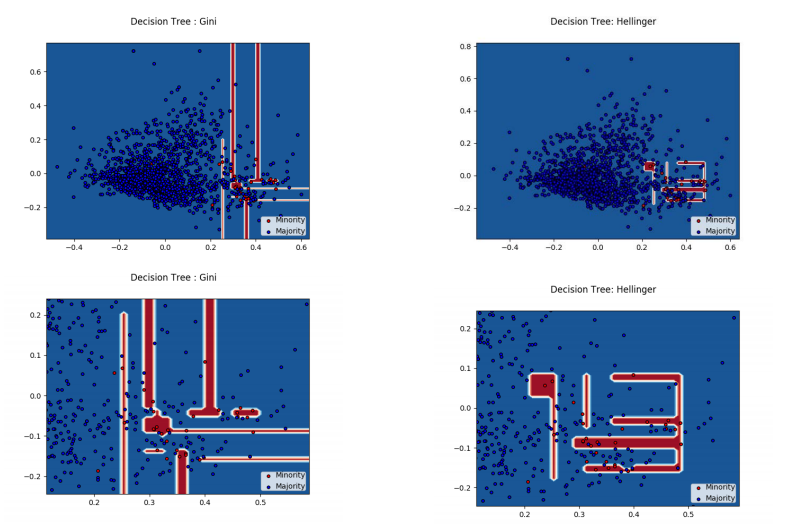
\includegraphics[width=100mm]{imagenes/hellinger-example.png}
	\label{fig:25}
	\caption{Ejemplo comportamiento algoritmo.}
\end{figure}
\verticalspace

Otra posible solución es modificar el peso asociado a clasificar mal un elemento, dando un peso mayor a clasificar mal un elemento de la clase minoritaria que de la mayoritaria, de forma que cuando se entrena el modelo intenta minimizarse el coste. El peso asociado a cada fallo se almacena en la matriz de costes, dicha matriz puede ser calculada con diferentes heurísticas o aportada por un experto en el problema que se plantee. El la siguiente imagen se muestra un ejemplo del uso de la matriz de costes para un clasificador simple.\newline

\begin{figure}[h]
	\centering
	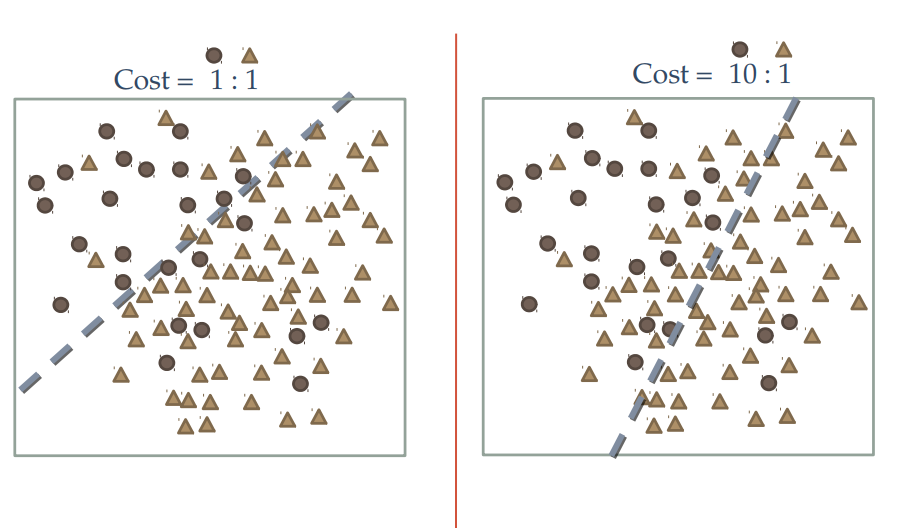
\includegraphics[width=90mm]{imagenes/cost-sentitive.png}
	\label{fig:26}
\end{figure}
\verticalspace

Existen dos formas de usar la matriz de costes, la primera es integrar el uso de la matriz dentro del algoritmo, lo que significa que hay modificarlo para que use dicha matriz; la segunda forma es preprocesando los datos de entrada asignándole un peso o asignando a cada elemento la clase que se cree que tendrá menor coste (para ello se hace uso del Teorema de Bayes).
\subsection{Técnicas basadas en la modificación del conjunto de datos}
La idea de este tipo de técnica es manipular la distribución de los datos con los que entrena el clasificador, para ello se añaden o suprimen elementos del conjunto de datos. Cuando se añaden elementos, se llama “oversampling” y cuando eliminan “undersampling”; dependiendo del problem se puede usar una de estas técnicas o ambas.\newline
\newpage
\begin{figure}[h]
	\centering
	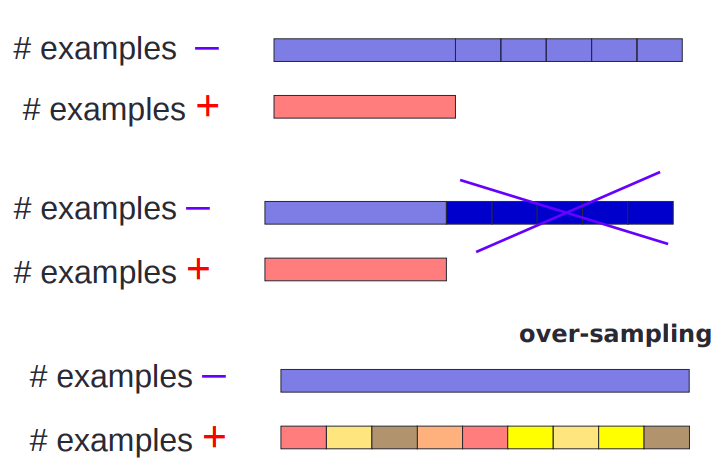
\includegraphics[width=110mm]{imagenes/oversampling_undersampling.png}
	\label{fig:27}
\end{figure}
\verticalspace

Un ejemplo clásico de algoritmo de undersampling es Tomek Links; este algoritmo elimina elementos de la clase mayoritaria que sean fronterizos con elementos de la clase minoritaria; para ello calcula las parejas de elementos de clases diferentes que estén a la distancia mínima entre ellos, es decir, que no haya ningún otro elemento dentro del conjunto de datos que su distancia hacia ese elemento sea menor; y elimina aquellos que sean de la clase mayoritaria. En la siguiente imagen se muestra un ejemplo del uso de este algoritmo.\newline


\begin{figure}[h]
	\centering
	
\includegraphics[width=120mm]{imagenes/tomek-example.png}
	\label{fig:28}
	\caption{Ejemplo funcionamiento algoritmo Tomek-Links.}
\end{figure}
\verticalspace

Otros métodos de undersampling son OSS, CNN y combinaciones de ellos. El problema del undersampling es que al eliminar elementos de la clase mayoritaria hace que cierta información se pierda, y dicha información puede ser importante al evaluar.\newline

Un algoritmo clásico de oversampling es SMOTE, este algoritmo crea nuevas instancias usando una combinación de K instancias de la clase minoritaria que sean vecinas. En la siguiente imagen se muestra un ejemplo del funcionamiento del SMOTE.\newline

\begin{figure}[h]
	\centering
	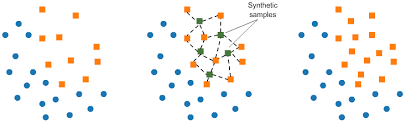
\includegraphics[width=120mm]{imagenes/smote-example.png}
	\label{fig:29}
	\caption{Ejemplo funcionamiento algoritmo SMOTE.}
\end{figure}
\verticalspace

Otros algoritmos de oversampling son modificaciones de SMOTE, como por ejemplo Borderline-SMOTE (centrado en la generación de instancias en la frontera), ADASYN, etc.\newline

El problema del oversampling es que pueden generalizar demasiado la clase minoritaria y provocar ruido en el conjunto de datos.

\subsection{Otros enfoques}
Una última opción para paliar el desbalanceo sin implicar modificaciones de los algoritmos o del subconjunto de datos, esta es el uso de modelos ensemble; los modelos ensemble son aquellos que están formados por varios modelos más simples, para ello, los modelos simples se entrenan con un subconjunto de los datos, de forma que en esos subconjuntos el desbalanceo no tiene porque ser tan grande. Para elegir una clase, los modelos ensemble pueden combinar los resultados de los modelos simples ( para problemas de regresión ) o mediante voto. Un ejemplo de modelo ensemble es RandomForest.